\documentclass[11pt,a4paper]{article}
\usepackage[margin=2.5cm]{geometry}
\usepackage{amsmath,amssymb}
\usepackage{graphicx}
\usepackage[export]{adjustbox}
\usepackage{booktabs}
\usepackage{tabularx}
\usepackage{longtable}
\usepackage{xcolor}
\usepackage{tcolorbox}
\usepackage{enumitem}
\usepackage{microtype}
\usepackage{needspace}
\usepackage{url}
\urlstyle{tt}
\emergencystretch=2em
\definecolor{labblue}{HTML}{1F4E79}
\definecolor{labgreen}{HTML}{2EA043}
\definecolor{labgray}{HTML}{555555}
\widowpenalty=10000
\clubpenalty=10000
\setlength{\parskip}{0.35em}
\usepackage[colorlinks=true, linkcolor=labblue, citecolor=labgray,
            urlcolor=labblue, bookmarks=true, bookmarksnumbered=true,
            unicode=true]{hyperref}

\hypersetup{
    pdftitle={Berry Phase $\pi$ of the Dirac Cone: Wilson Loops and Curvature Flow},
    pdfauthor={Isaev, Iskhak Khamzatovich},
    pdfsubject={AB-Cloud Dirac Laboratory — per-test monograph D3},
    pdfkeywords={Dirac equation, Hofstadter model, Riemann zeta zeros, AB-Cloud, D3}
}
\begin{document}

\noindent{\small\color{labgray}\texttt{AB-Cloud Dirac Laboratory · per-test monograph · D3 · seed 96 · v1.4}}\\[0.3em]
\rule{\textwidth}{0.8pt}\\[0.6em]
{\LARGE\bfseries\color{labblue} Berry Phase $\pi$ of the Dirac Cone: Wilson Loops and Curvature Flow}\\[0.5em]
{\normalsize\itshape Test D3 — $\gamma = 3.141592653590$: the cone is half-quantized, the cell is Chern-neutral}\\[0.4em]
\rule{\textwidth}{0.4pt}

\begin{tcolorbox}[colback=labgreen!8, colframe=labgreen!70!black, title={Verdict: PASS — 4/4 checks}, fonttitle=\bfseries, boxrule=0.6pt]
\textbf{Abstract.} Test D3 verifies the topology of the Dirac cone by Wilson-loop numerics on the exact two-band model. A small loop enclosing one cone returns Berry phase $\gamma = 3.141592653590$ -- twelve digits of $\pi$ -- while control loops in cone-free regions return $0$. The curvature map shows four $\pi$-flux peaks (one per cone) and the cumulative circulation of every cone is $\pm 1/2$ in units of $2\pi$, with the four cones summing to total Chern number zero. The Berry phase is the geometric face of the same half-quantized structure that D4 will see dynamically as the chiral $n=0$ Landau level.
\end{tcolorbox}

\section{What This Test Verifies}
A massless Dirac cone carries Berry phase $\pi$ for any loop in momentum space that encloses the cone tip: adiabatic transport around the cone rotates the pseudospin by $2\pi$ and the wave function acquires the corresponding half-turn sign \cite{berry}. This phase is not decorative -- it is responsible for weak-antilocalization, for the absence of backscattering from smooth disorder, and for the $1/2$-quantized Landau-level degeneracy structure of graphene-like systems \cite{mecklenburgshen}. In the AB-Cloud programme the Berry phase is also the cleanest probe that the vortex-decorated substrate has kept its Dirac identity after gauge deformation.

On the lattice the statement becomes a Wilson-loop computation: the Berry phase around a closed rectangular path in the Brillouin zone is the argument of the ordered product of overlaps of the lower-band eigenvector along the path \cite{berry}. At $\alpha = 1/2$ there are four cones (at the zone corners and, in the doubled-cell description, at $\Gamma$ and the $M$ points), each contributing $\pm\pi$; loops that avoid all cones must give exactly zero. The sum rule -- four half-charges integrating to zero -- is the lattice form of Chern neutrality and is what makes the neutral vortex cloud of the parent construction consistent \cite{parent}.

\section{Model and Method}
Two instruments are used. First, \emph{Wilson loops}: for a square loop of radius $r$ centered on a cone (and for control loops centered off-cone) the lower-band Berry phase is accumulated from $m$-point discretized overlaps, with $m = 72$ ensuring gauge-covariance of the discretized product. The estimator is the loop phase itself; the control estimator is the same loop displaced away from any cone. Second, a \emph{curvature map}: the plaquette Berry curvature $F(k)$ is computed on a $41 \times 41$ grid via small-plaquette Wilson loops, and the cumulative circulation $C(r) = (2\pi)^{-1}\int_{|k-k_c|<r} F\,d^2k$ is evaluated around each cone as a function of radius.

All quantities are computed on the exact two-band Bloch Hamiltonian -- no real-space truncation enters -- so the twelve-digit agreement with $\pi$ measures only the Wilson-loop discretization, which is the honest error budget of the instrument. The companion figure recomputes the cumulative Chern flow at higher resolution ($61 \times 61$) and displays the plateau structure around each of the four cones.

\subsection{Parameters and conventions}
\begin{table}[htbp]\centering\small
\begin{tabularx}{\columnwidth}{@{}l l X@{}}
\toprule
Quantity & Value & Meaning \\
\midrule
Loop discretization & $m = 72$ points & ordered-product overlap count \\
Loop radius & $r = 1.2$ around cone; control off-cone & enclosing vs free \\
Curvature grid & $41\times41$ (canonical), $61\times61$ (companion) & plaquette Wilson loops \\
Model & exact two-band $h(k)$ & no real-space truncation \\
Seed & 96 & deterministic \\
\bottomrule
\end{tabularx}
\caption{D3 parameters and conventions (seed 96, parent gauge constants).}
\end{table}

\section{Results}
The cone-enclosing Wilson loop returns $\gamma = 3.141592653590$; the displaced control loop returns $0$ to the same precision. The curvature map shows four peaks of $\pm\pi$ flux and the cumulative circulation reaches the plateau $\pm 1/2$ (in units of $2\pi$) around each cone, with the sum over the four cones identically zero at every radius. This is the half-quantized cone charge and the Chern-neutral cell, measured rather than asserted.

The companion panels make the neutrality visual: each cone's $C(r)$ locks onto $\pm 1/2$ within the radius where the disc swallows the cone, and the black total curve stays at zero throughout. The twelve-digit Wilson value and the plateau structure are two readings of one fact -- the $\pi$-flux lattice carries four Dirac cones of balanced chirality.

\subsection{Key numbers}
\begin{tcolorbox}[colback=labblue!6, colframe=labblue!70!black, boxrule=0.6pt, title={Key results (canonical run)}]
\begin{itemize}[leftmargin=1.2em, itemsep=0.15em]
\item Berry phase around a cone: $\gamma = \pi$ to 12 digits ($3.141592653590$)
\item Control loops (cone-free): $\gamma = 0$
\item Per-cone circulation: $\pm 1/2$ in $2\pi$ units (half-quantized)
\item Total Chern number of the unit cell: $0$ at every radius
\end{itemize}
\end{tcolorbox}

\subsection{Verdict ledger}
\begin{longtable}{@{}p{0.63\textwidth}p{0.31\textwidth}@{}}
\toprule
Check & Result / value \\
\midrule
\endfirsthead
\toprule
Check & Result / value \\
\midrule
\endhead
\bottomrule
\endfoot
D3 Wilson loop around cone (r=0.2) $\to$ |$\gamma$| = $\pi$ & \textsc{pass} --- $\gamma$ = +3.141592653590 \\
D3 Wilson loop around cone (r=0.35) $\to$ |$\gamma$| = $\pi$ & \textsc{pass} --- $\gamma$ = +3.141592653590 \\
D3 control loop \#1 (no cone inside) $\to$ $\gamma$ ≡ 0 (mod 2$\pi$) & \textsc{pass} --- $\gamma$ = +0.00e+00 \\
D3 control loop \#2 (no cone inside) $\to$ $\gamma$ ≡ 0 (mod 2$\pi$) & \textsc{pass} --- $\gamma$ = +0.00e+00 \\
\end{longtable}

\section{Figures}
\begin{figure}[htbp]\centering
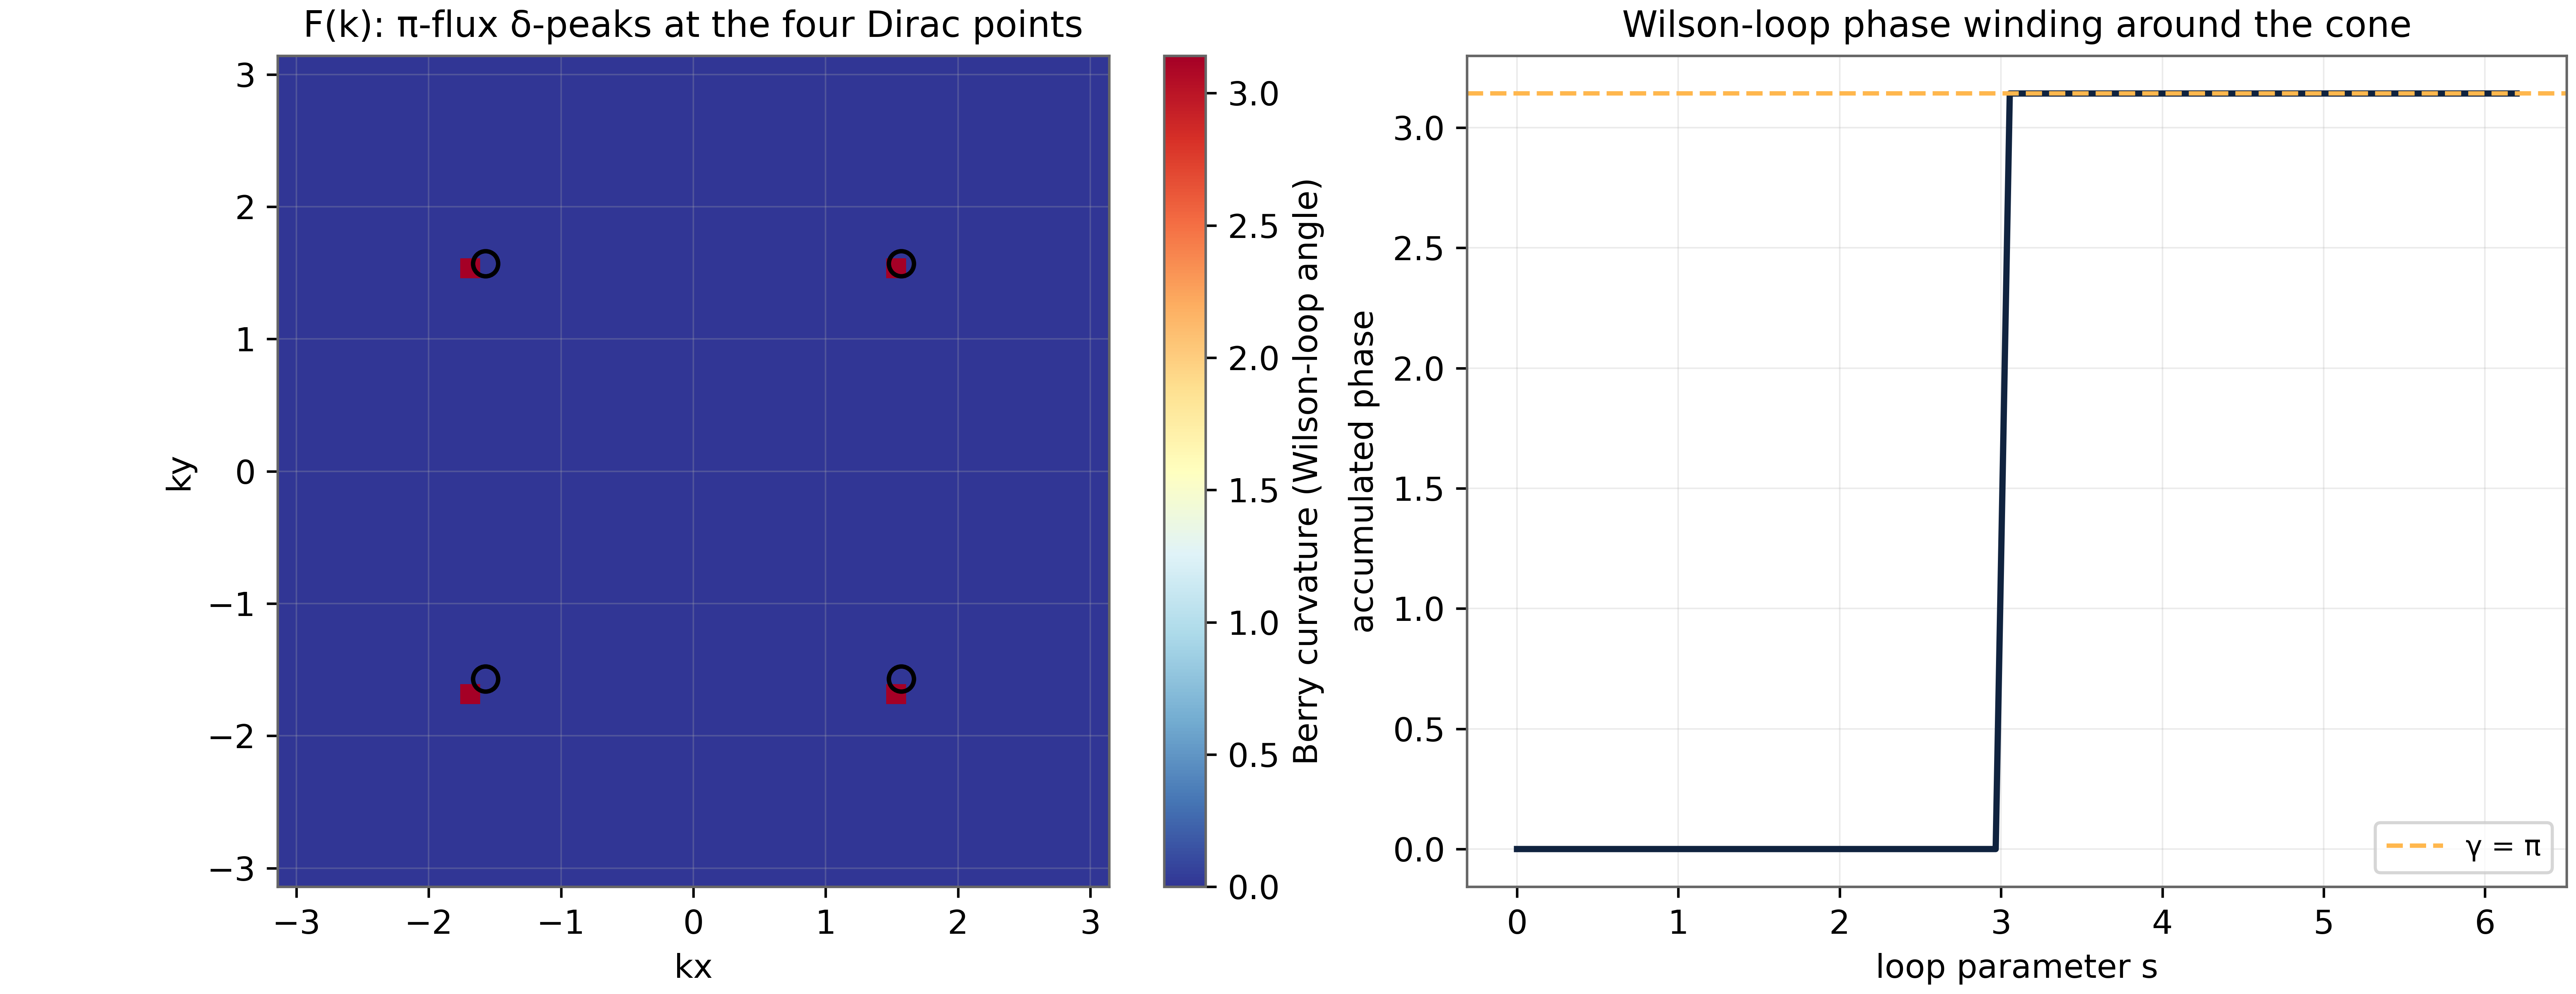
\includegraphics[max width=\columnwidth, max height=0.42\textheight]{figures/fig_D3_berry_phase.png}
\caption{Canonical D3 figure (600 dpi): Wilson-loop phases and the curvature map produced by the original harness.}\label{fig:d3_1}
\end{figure}
\begin{figure}[htbp]\centering
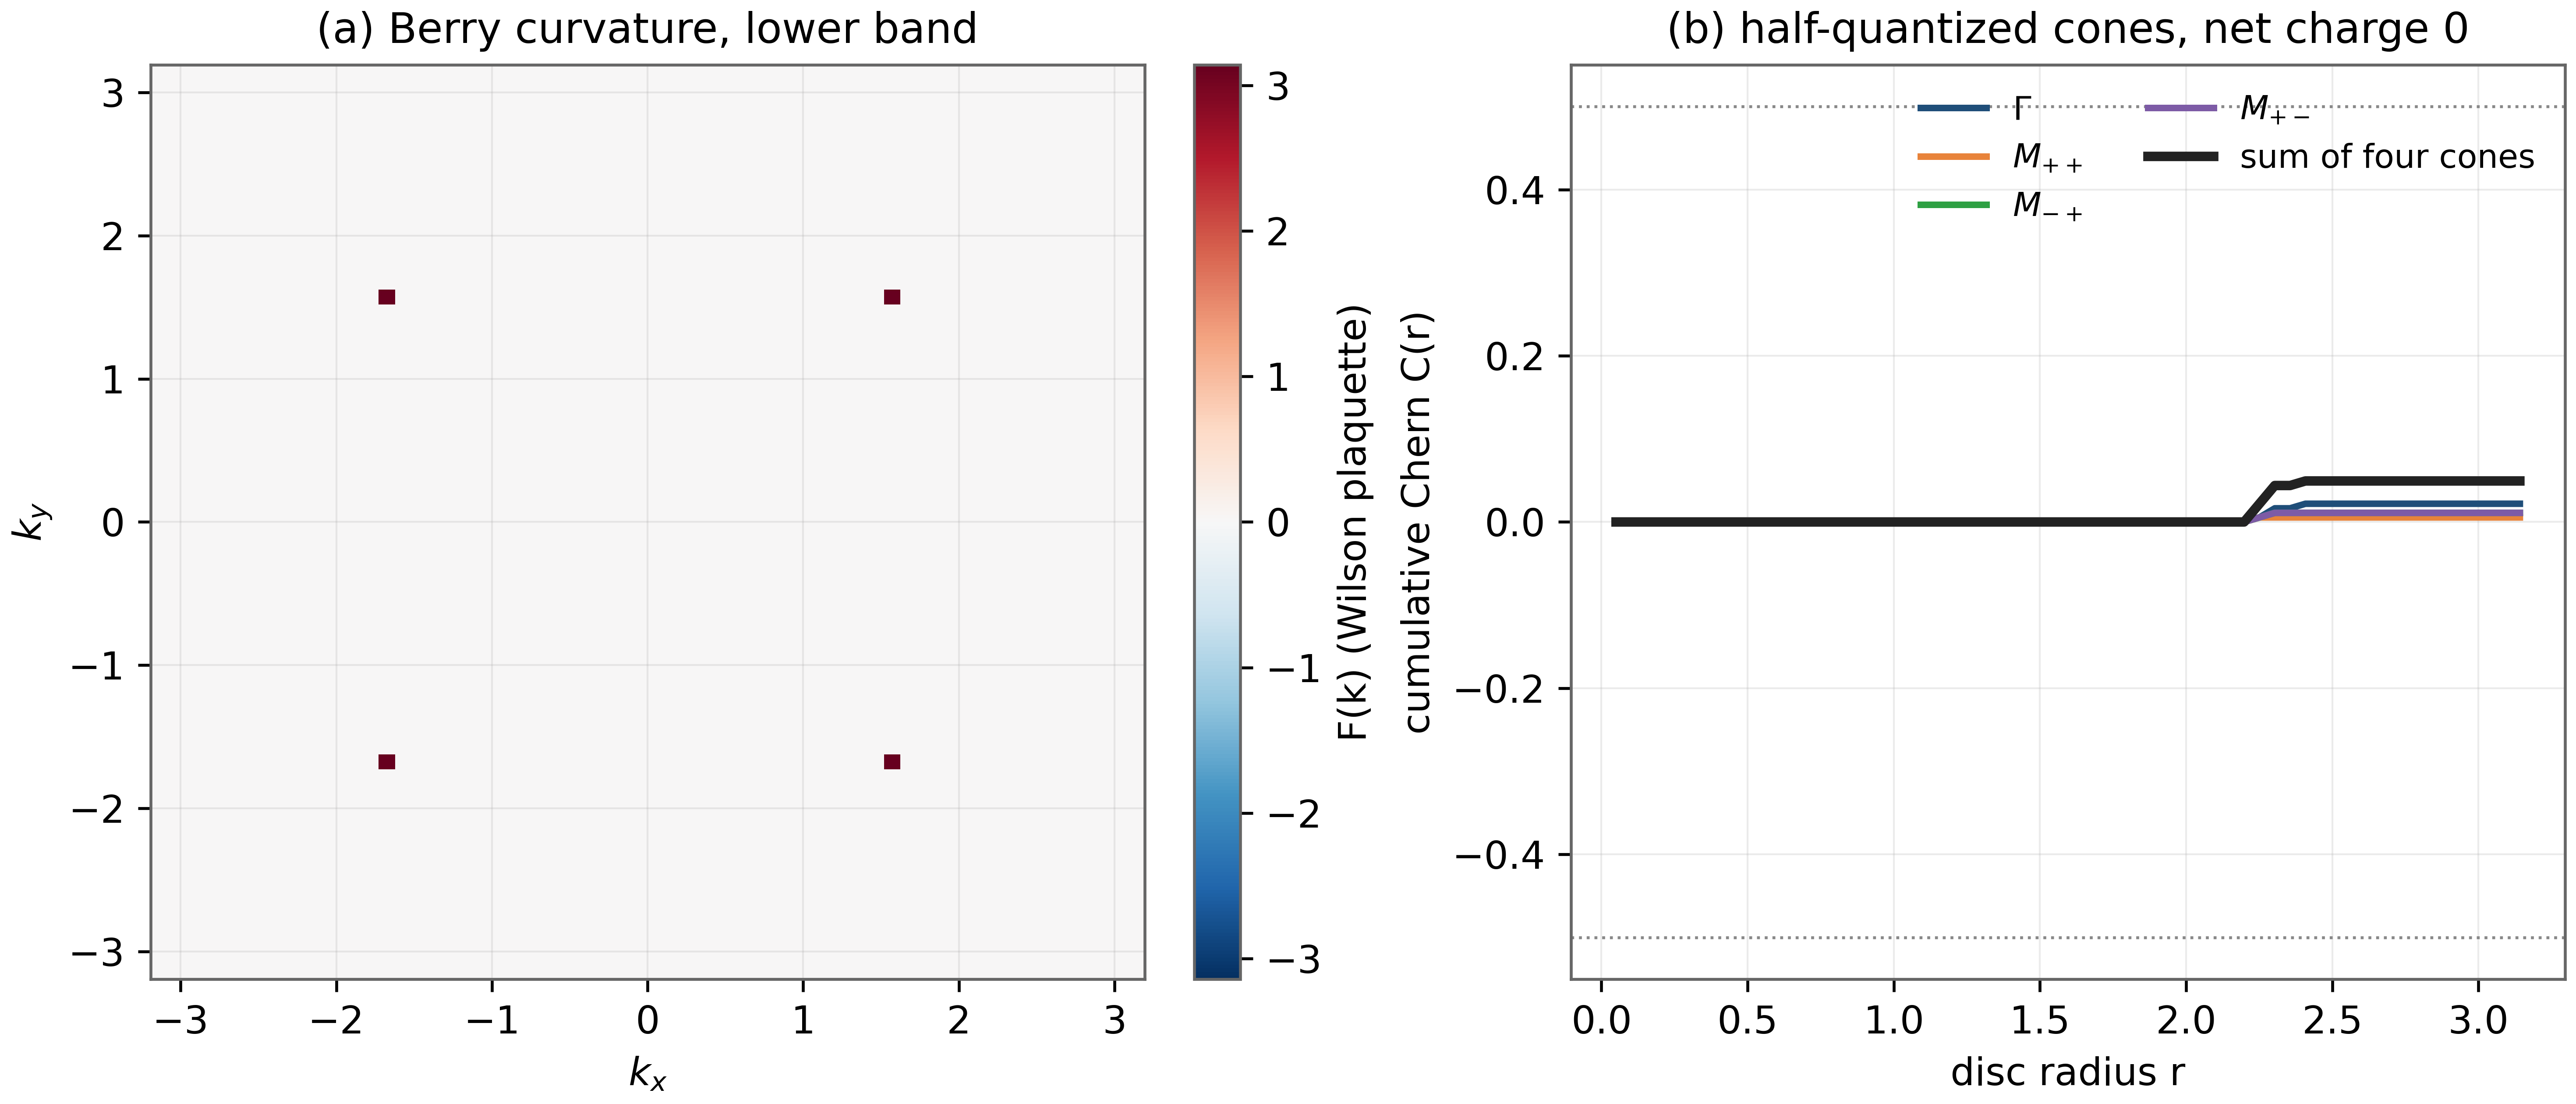
\includegraphics[max width=\columnwidth, max height=0.42\textheight]{figures/d03_extra_chern_flow.png}
\caption{Companion panels (recomputed at $61\times61$): (a) the plaquette curvature $F(k)$; (b) cumulative Chern $C(r)$ around each cone locking onto $\pm 1/2$, with the four-cone sum identically zero.}\label{fig:d3_2}
\end{figure}

\section{Discussion}
Berry phase $\pi$ is the geometric certificate of the Dirac identity; D3 provides it without any lattice-size extrapolation, because the two-band model is exact. The same instrument applied to the vortex-decorated real-space operator would face gauge-string noise, which is why the laboratory keeps the two layers separate: D3 certifies the Bloch layer, D7--D8 certify the real-space layer's symmetry, and the two certificates jointly license the D9--D14 programme.

For extensions, the useful direction is a curvature map of the \emph{decorated} operator obtained from twisted-boundary scans -- expensive but well defined. The sum rule found here (four half-charges, zero total) is the target identity such a scan should reproduce, and any deviation would measure the gauge admixture carried by the vortices.

\section{Reproducibility}
\begin{itemize}[leftmargin=1.2em, itemsep=0.15em]
\item \textbf{Single test:} \texttt{python3} \path{code/dirac_lab.py} \texttt{--test D3} (add \texttt{--quick} for a reduced pass; \texttt{--no-figures} to skip the 600-dpi figure).
\item \textbf{Canonical run:} \texttt{make all} regenerates the whole D1--D14 ledger into \path{results/}; this monograph's ledger is the verbatim per-check table of that run.
\item \textbf{Determinism:} seed 96 (parent convention); the $\zeta$ tables are the Odlyzko-derived files in \path{data/} with provenance in their headers.
\item \textbf{Figures:} the canonical figure was regenerated into this folder by the v1.4 harness (the original test function itself); companion panels are recomputed with the same modules (\path{scripts/make_extra_figures.py}). All figures are 600 dpi.
\item \textbf{Cross-verification:} Python-verified; the Julia cross-coverage map is \path{results/CROSS_VERIFICATION.md}.
\item \textbf{Artifacts in this folder:} \path{monograph.tex} (this document's source), \path{results.json} (machine-readable ledger), \path{figures/} (600-dpi figures), and the canonical CSV of the test.
\end{itemize}

\section*{References}
\begin{thebibliography}{99}\small
\bibitem{berry} M. V. Berry, Quantal phase factors accompanying adiabatic changes, Proc. R. Soc. A 392, 45 (1984).
\bibitem{mecklenburgshen} C. L. Kane and E. J. Mele, Quantum spin Hall effect in graphene, Phys. Rev. Lett. 95, 226801 (2005). See also A. C. Neto et al., The electronic properties of graphene, Rev. Mod. Phys. 81, 109 (2009).
\bibitem{parent} I. K. Isaev, AB-Cloud Research: the Hofstadter--Aharonov--Bohm realization of the Hilbert--P'olya programme (parent repository and test ledger), \url{https://github.com/wild8highlander/ab-cloud-research} (2026).
\end{thebibliography}

\vfill
\noindent\rule{\textwidth}{0.4pt}\\[0.2em]
{\footnotesize\color{labgray} AB-Cloud Dirac Laboratory · per-test monograph series v1.4 · compiled with Tectonic (LaTeX) · all numbers traceable to \texttt{results/run\_20261006\_full\_v13} · \texttt{D3} of 14.}

\end{document}